%%%%%%%%%%%%%%%%%%%%%%%%%%%%%%%%%%%%%%%%%%%%%%%%%%%%%%%%%%%%%%%%%%%%%%%%%%%%%%%%%%%%
% Template for STAT 548 Qualifying Paper Report
% Author: Ben Bloem-Reddy <benbr@stat.ubc.ca>
% Revised: Daniel J. McDonald <daniel@stat.ubc.ca>
% Date: 26 August 2024
%%%%%%%%%%%%%%%%%%%%%%%%%%%%%%%%%%%%%%%%%%%%%%%%%%%%%%%%%%%%%%%%%%%%%%%%%%%%%%%%%%%%

% Note: You will get an empty bibliography warning when compiling until you include a citation.

\documentclass[12pt]{article}
\usepackage[commenters={JZ,DJM}]{shortex} % replace OA with your initials
\usepackage[round]{natbib}
\usepackage[margin=2.5cm]{geometry}
\newcommand{\email}[1]{\href{mailto:#1}{#1}}

% minor adjustments to ShorTeX
\let\argmin\relax\DeclareMathOperator*{\argmin}{argmin}
\let\argmax\relax\DeclareMathOperator*{\argmax}{argmax}
\DeclareMathOperator*{\minimize}{minimize}
\DeclareMathOperator*{\maximize}{maximize}
\DeclareMathOperator{\subjto}{\ \text{subject to}\ }
\renewcommand{\top}{\mathsf{T}}
\renewcommand{\d}{\mathsf{d}}

\graphicspath{{fig/}}



%%%%%%%%%%%%%%%%%%%%%%%%%%%%%%%%%%%%%%%%%%%%%%%%%%%%%%%%%%%%%%%%%%%%%%%%%%%%%%%%%

% your title/author/date information go here
\title{How to Best Model Epidemics: \\
Comparing Reproduction Number and Growth Rate \\
\large STAT 548 Qualifying Paper Report} % replace with your title, a meaningful title
\author{Justin J. Zhang} % replace with your name
\date{\today} % replace with your submission date


% start of document
\begin{document}
\maketitle
\newpage
  \section{Summary of Paper}
    As the world moves forward from the Coronavirus pandemic, the question for epidemiologists and policy makers is how to 
    best prevent the spread of future novel viruses. A major step towards epidemic prevention is the accurate statistical 
    modelling of epidemic growth. \citep{Parag2022}, henceforth denoted PTD, aim to tackle this problem by examining 
    two popular statistics of epidemic growth: the instantaneous reproduction number $R_t$, 
    and the instantaneous growth rate $r_t$. 

    For a long time, $R_t$ has been the preeminent statistic for health professionals. However, it requires model assumptions, which
    may have drastic effects on real-world policy if misspecified.
    Sceptics argue $r_t$ is a better statistic as it does not require explicit
    model assumptions and is therefore more informative \citep{Pellis2022}. PTD aim to refute this claim by showing that there is a relationship 
    between $\hat{R}_t$ and $\hat{r}_t$ that does not rely on model assumptions. 
    This section covers the relevant theory and methods behind these statistics, the main contributions from PTD, 
    and the limitations in both the paper and general epidemic modelling.

    \subsection{Relevant Theory}
      To start, we define the notation used in PTD. Let $t= 1,\dots,T$ be a sequence of discretized time-steps, which in PTD
      represents days. Let $I_t$ denote the $\textit{incidence of infection}$ (denoted as incidence) at time $t$, representing the number of new infections.
      Call $\{I_1,\dots,I_T\}$ the $\textit {incidence curve}$. 
      Let $W = \{w_j\}_{j=0}^\infty$ be the $\textit{generation time distribution}$, denoted GTD, so that $w_j$ represents
      the probability mass that an infected individual will generate a secondary infection in exactly $j$ days. In practice, 
      we cannot observe incidence, so the GTD is often approximated by the \textit{serial interval distribution}, which uses reported cases
      in place of infections \citep{Cori2013}. In this paper, we will use GTD. 
      
      \paragraph{Modelling $R_t$} The $\textit{instantaneous reproduction number}$, $R_t$, measures the mean number of secondary infections generated from each
      infected individual at time $t$, 
      with a value greater than 1 indicating a growing epidemic. The renewal model \citep{Fraser2007} 
      in \cref{eq: Rt} is used to estimate $\hat{R}_t$. We first compute the $\textit{total infectiousness } \Lambda_t$, 
      the number of new infections at time $t$ caused by previous incidences with respect to GTD. 
      $\hat{R}_t$ is then the multiplier of $\Lambda_t$ to achieve the expected incidence at time $t$, hence the 
      \textit{instantaneous} reproduction rate. 

      \begin{equation} \label{eq: Rt}
        \mathbb{E}(I_t) = \Lambda_t R_t, \qquad \Lambda_t = \sum_{j = 1}^{t - 1} I_{t - j} w_j \implies R_t =
         \frac{\mathbb{E}(I_t)}{\sum_{j = 1}^{t - 1} I_{t - j} w_j}
      \end{equation}

      PTD use Bayesian estimation to estimate $\hat{R}_t$ from $I_1,\dots,I_t$. The prior $\pi(R_t)$ is assumed to be from
      the gamma distribution, and the likelihood $f(I_t \ | \ I_{t-1},\dots,I_1, W, R_t)$ assumed to be Poisson distributed. 
      These choices are due to convenience, though the Poisson assumption suffers from overdispersion in practice.
      The posterior $\pi(R_t \ | \ I_{t-1},\dots,I_1, W, I_t)$ is then derived to also be from a gamma distribution, 
      and $\hat{R}_t$ is estimated as the posterior mean (\citep{Cori2013} and \cref{app: bayes}).

      \paragraph{Modelling $r_t$} The \textit{instantaneous growth rate}, 
      $r_t$, has increased in popularity due its lack of distributional assumptions in comparison with $R_t$. $\hat{r}_t$ is estimated directly from a 
      smoothed incidence curve, with respect to a log-differentiable function $\mathbb{S}_t$, as seen in the left side of 
      \cref{eq: rt}. As an example of a smoothing function, PTD champion the
      usage of the \textit{Savitsky-Golay} (SG) filter, a local interpolation method. A SG filter of dimension $m$, with 
      $m$ odd, given in the right side of \cref{eq: rt}, performs polynomial interpolation of degree $p$, with $p \leq m$, on a 
      moving window $t - \frac{1 - m}{2}, \dots, t + \frac{m  - 1}{2}$ \citep{SavitzkyGolay1964}. The log derivative is then taken with respect to the fitted polynomials,
      and $\hat{r}_t$ is its value at $t$. Though no model is used, $\hat{r}_t$ is still considered an estimate in terms of a given smoothing function,
      which shows that the choice of $\mathbb{S}$ functions as a sort of assumption. 
      \begin{equation} \label{eq: rt}
        r_t = \frac{\d \log{\mathbb{S}_t}}{\d t}, \qquad S_t = \sum_{j = (1 - m)/2}^{(m  - 1)/2} I_{t + j}\alpha_j
      \end{equation}
      
      \paragraph{Connecting $\hat{R}_t, \hat{r}_t$} Under the assumption of a GTD for $r_t$ there is an explicit link between $\hat{r}_t$ 
      and $\hat{R}_t$ through its moment generating function $\mathbb{M}_W(I)$
      \citep{WallingaLipsitch2006}. The general formulation, called the Lotka-Euler equation,
      as well a specific instance where $W$ is taken from a 
      $\text{Gamma}(\alpha, \beta)$ distribution is given in \cref{eq: rt-Rt}. The equation is derived by assuming 
      exponential growth for the incidence at a rate of $\hat{r}_t$, that is $I_t = I_{t-j} e^{j \hat{r}_{t}}$
      (see \cref{app: rtRt}). This gives a bijective relation to obtain $\hat{r}_t$ directly from an estimate of $\hat{R}_t$. 
      \begin{equation} \label{eq: rt-Rt}
        \hat{R}_t \mathbb{M}_w(-\hat{r}_t) = 1, \qquad \hat{r}_t = \beta(\hat{R}_t^{\frac{1}{\alpha}} - 1)
      \end{equation}

    \subsection{Main Contributions}
      We have seen that under distributional assumptions, $\hat{r}_t$ is connected to $\hat{R}_t$. 
      PTD show that there is additionally a non model-dependent connection between 
      $\hat{R}_t$ and $\hat{r}_t$ that refutes the notion that
      the distributional assumptions on $\hat{R}_t$ make it less informative \citep{Pellis2022, DushoffPark2021}.
      They illustrate their claim through a simulated case study shown in \cref{fig: paper} (note that PTD use \textit{EpiEstim} \citep{Nash2023} 
      as opposed to \textit{rtestim}), though it is never rigorously proven. To do so, they estimate $\hat{r}_t$ once
      using SG filters as in \cref{eq: rt} and again using $\Lambda_t$ as a smoothing function.

      The results show that both methods accurately model $r_t$, highlighting an explicit link between
      the distributional assumptions for $\hat{R}_t$ and choice of smoothing function for $\hat{r}_t$. In fact PTD show $\Lambda_{t+\tau}$ is approximately equal to $S_t$ 
      for $\tau \approx \mathbb{E}(W)$. Both are functions of the daily incidence, and so under correct model specification the
      estimated coeffcients $\alpha_j$ determine it's own distribution. For a reasonable GTD, $w_j$ will be near 0 for $j > 2\tau = 2\mathbb{E}(w)$,
      and so with $m = 2\tau - 1$, \cref{lambda SG} shows that GTD is functionally a smoothing filter through $\Lambda_t$ by setting the 
      coefficients $w_j = \alpha_{\tau - j}$.
      \begin{equation} \label{lambda SG}
        \Lambda_{t+\tau} = \sum_{j = 1}^{t + \tau - 1} I_{t + \tau - j}w_j  
        \approx \sum_{j = 1}^{2\tau - 1} I_{t + \tau - j}\alpha_{\tau -j}
        \approx \sum_{j = 1 - \tau}^{\tau - 1} I_{t - j} \alpha_{-j}
        = \sum_{j = 1 - \tau}^{\tau - 1} I_{t + j} \alpha_{j}
      \end{equation}
      
      \cref{lambda SG} shows that the smoothing function $\mathbb{S}_t$
      as chosen in \cref{eq: rt} has underlying distributional assumptions. That is, even when a GTD is not imposed on the incidence curve,  
      i.e. no model assumptions, 
      the estimated filter coeffcients $\alpha_j$ themselves form an arbitrary kernel for each $S_t$ that is similar to a GTD. 
      When the filter is taken over a relatively large moving window, these coefficients will not substantially change between time points. 
      It is worthwile to mention that PTD only show this connection for the SG filter as a smoothing function, not for smoothing
      functions in general. 
      
      PTD try to use this paper to highlight when each statistic would be more informative.
      One benefit of estimating $r_t$ is performance when the GTD 
      is misspecified. $\hat{R}_t$ is derived immediately from $W$ and so naturally has high bias under misspecification. 
      However, using \cref{eq: rt-Rt} to compute $\hat{r}_t$ from the poorly estimated $\hat{R}_t$ 
      still recovers an estimate of $\hat{r}_t$ with low bias (see \cref{fig: misspec}). Under good model specification, 
      PTD say that $\hat{R}_t$ is a more informative estimate of epidemic growth 
      since $\hat{r}_t$ is estimated from it. In general, $\hat{R}_t$ quantifies the number of
      secondary transmissions that need to be prevented on average to slow the pandemic, which is a determining factor in 
      epidemic policy and vaccine coverage. $\hat{r}_t$ measures the speed of epidemic growth, 
      and gives metrics such as doubling time, which is a determining factor in intervention planning. 

    \subsection{Limitations}
      There are a number of limitations to the work in PTD, both in their analysis
      and its ability to accurately model epidemics. 

      \paragraph{Case vs Incidence data} One primary issue is that 
      incidence data is incredibly difficult to measure. Since we estimate it from case reports, it is a right censored estimate, 
      i.e. requiring future case numbers and incubation times to accurately measure. 
      In some cases, it will also be left censored if baseline infections
      from the start of an epidemic are not known \citep{Fraser2007}. 
      Furthermore, a decent percentage of incidences are never reported,
      and so the true incidence is impossible to know. This adds a layer of data-dependent irreducible variance to 
      $\hat{R}_t$ and $\hat{r}_t$, an issue PTD never mention ways to mitigate. 
      One possible solution \citep{Comiskey2021} is to estimate the distribution of incubation time, 
      $\{\beta_i\}_{i=1}^\infty$, using reported case data $C_t$ and true incidence numbers from wastewater collection within neighbourhoods. 
      We can then back-calculate incidence through the formula $\hat{I}_t = \sum_{i=0}^\infty \hat{\beta}_i C_{t+i}$. 
      The hope is that the additional variance from an extra layer of prediction is less than the reduction in variance on the main
      model. 
      
      \paragraph{Outside Factors} A major assumption of the renewal model is that incidence propagates forward at the same rate
      regardless of the time, i.e. they assume the same population susceptibility. 
      This is unlikely to hold because of human behaviour and government intervention. Policies
      like vaccine mandates and quarantines drastically drop the number of suscetible individuals. 
      During extended quarantines, people will slowly become more willing to break rules, which in turn increases the susceptible population.
      These effects cannot be fully captured in the GTD and so $\hat{R}_t$ estimates will not account for them. 
      To account for changes in susceptibility, we can assume incidence is distributed based on $\lambda_t \Lambda_t R_t$
      where $\lambda_t$ measures deviation from baseline susceptibility. Changes in human movement like lockdowns
      can be estimated from movement data, i.e. number of people at places like grocery stores and events, though vaccine effect
      is more difficult to model. The \textit{case reproduction number}, $R^c_t$, which measures the average number of secondary infections 
      \textit{over a lifetime}, implicitly accounts for these changes, but is a
      retrospective statistic since it requires future incidence numbers \citep{Cori2013}. PTD fail to measure how
      $\hat{r}_t$ performs when susceptibility changes, though the GTD-independent estimates will likely still be good due to being
      estimated based on actual incidence. They do off-handedly mention the
      \textit{Susceptible-Infectious-Recovered} model that groups people into these three categories, but it is often an
      oversimplication of true epidemic dynamics \citep{Lloyd2009}.  

      
      \paragraph{Issues with the Paper} The largest limitation with this paper is that PTD never discuss \textit{how} to use 
      $\hat{R}_t$ and  $\hat{r}_t$ together to
      understand epidemic dynamics. For a paper who's primary objective is to clarify the understanding of these statistics, 
      there are no concrete applications beyond ``use both". Furthermore, most of the theory is hand-waved, which is okay
      because they reference supplementary papers, but makes it more difficult for readers to both understand their assumptions and follow
      their logic. In summary, PTD do a sufficient job to compare $\hat{R}_t$ and $\hat{r}_t$, and refute the thought that the lack
      of distributional assumptions in $\hat{r}_t$ is an inherent advantage. Beyond that they have not developed any novel 
      methods or ideas that can be applied to real-world epidemiological modelling. 

      \newpage

  \section{Mini-Proposals}
      In the previous section, we discussed PTD's claim that the smoothing function assumed to estimate $r_t$ is itself an implicit
      distributional assumption, which refutes claims that $r_t$ is a better statistic to measure epidemics \citep{Pellis2022}. 
      The logical next step is to consider whether we can still estimate $r_t$ without the use of any explicit smoothing functions.
      In this section we propose a method to smooth the estimators $\hat{r}_t$ directly rather than smoothing the
      incidence itself (e.g. SG filter), thereby not using functional assumptions. 

      Recall that the incidence is assumed to come from a Poisson parameter. In \cref{eq: Rt} we took the rate as
      $\Lambda_t R_t$, however, since we are no longer applying distributional assumptions we simply
      use exponential growth, that is $I_t \ |\ I_{t-1} \sim \text{Poisson}(I_{t - 1}e^{r_t})$ where the parameter of interest is $r_t$.
      This is a \textit{Poisson many means model} where each observation $I_t$ has a different rate parameter. We also have the
      simplifying assumption of independence, which likely does not hold because $I_t$ is explicitly dependent on $I_{t - 1}$.
      The first naive method of estimation we would consider is to simply take the MLE.
      \begin{align} \label{rt: MLE}
          (\hat{r}_1^{MLE},\dots,\hat{r}_T^{MLE}) &= \argmax_{(r_1,\dots,r_T) \in \mathbb{R}^T} \mathcal{L}(r_1,\dots,r_T ; I_1,\dots,I_T) \\
          &= \argmax_{(r_1,\dots,r_T) \in \mathbb{R}^T} \prod_{t = 2}^T \frac{(I_{t - 1}e^{r_t})^{I_t} e^{-I_{t - 1}e^{r_t}}}{I_t!} \\
          &= \argmin_{(r_1,\dots,r_T) \in \mathbb{R}^T} \sum_{t = 2}^T -[I_t(\log{I_{t - 1}} + r_t) - I_{t - 1}e^{r_t}]
      \end{align}
      Deriving in terms of each $r_t$ and setting to 0 gives a set of solutions
      $\hat{r}_t^{MLE} = \log{I_t} - \log{I_{t - 1}}$. Note that for this paper, we assume that 
      $I_t > 0$ by increasing each $I_t$ by some small tolerance $\epsilon$ (say $\epsilon = 1$) so we can safely take logarithms.

      The MLE under Poisson assumption gives an unbiased estimator with respect to incidence, that is $E(I_{t - 1}e^{\hat{r}_t} \ |\ I_t) = I_t$. 
      However, since we have assumed independence, the risk of this set of estimators $\hat{r}_1^{MLE},\dots,\hat{r}_T^{MLE}$ under squared error is
      \begin{align}
        R(I_{-1}\hat{r}^{MLE}, I) = \sum_{t = 2}^T \mathbb{E}(I_t - I_{t - 1}e^{r_t})^2 = \sum_{t = 2}^T \text{Var}(I_t) = \sum_{t = 2}^T I_{t - 1}e^{r_t}
      \end{align}

      Here, $I_{-1}$ is the incidence vector shifted 1 day to the left, so that ${I_{-1}}_t$ matches $I_{t + 1}$. 
      Since incidence will be non-negative for non-trivial epidemics, and similarly growth rate will not be strictly negative, as $T \to \infty$, 
      this risk function will blow up to infinity. This is because each $\hat{r}_t^{MLE}$ is fit individually, 
      which gives unbiasedness but increases variance for $(\hat{r}_1^{MLE},\dots,\hat{r}_T^{MLE})$ as a whole. 
      Moreover, based on the incidence curve, we can very well get $\hat{r}_t^{MLE}$ jumping around, 
      leading to an incredibly unsmooth estimator, as shown in \cref{fig: smoothrt}. 
  
      Accordingly, our goal is decrease the estimator variance by inducing some level of bias. 
      Our proposed method is to add a smoothing function on the parameters themselves. This is opposed to 
      \cref{eq: rt} which smooths the data. The method is analogous to the \textit{rtestim} method of estimating $R_t$ \citep{Liu2024}.
      We are applying a penalty on the differences in growth rates and adding it to the Poisson loss
      from \cref{rt: MLE}. We get the smoothed estimator in \cref{rt: smooth}
      \begin{align} \label{rt: smooth}
          (\hat{r}_1^{\lambda},\dots,\hat{r}_T^{\lambda}) &= \argmin_{(r_1,\dots,r_T) \in \mathbb{R}^T} \sum_{t = 2}^T [I_{t - 1}e^{r_t} - I_t(\log{I_{t - 1}} + r_t)]
         + \sum_{t = 3}^T [\lambda_1 e^{(r_t - r_{t - 1})^2} + \lambda_2 e^{(r_t - 2r_{t - 1} + r_{t -2})^2}]
      \end{align}

      The corresponding derivative of this objective function is not directly solvable for $\hat{r}_t^{\lambda}$, 
      but note that it is a convex function (see \cref{app: convex}) so can be easily solved
      with pre-existing convex optimization methods.

      The solution to \cref{rt: smooth} will smooth the estimated parameters in 2 ways. The first penalty term controls
      the magnitude of the first difference in growth rates $r_t - r_{t - 1}$, which ensures there are no big jumps in growth rate between days. 
      The second penalty term controls
      the magnitude of the second differences $r_t - 2r_{t - 1} + 2r_{t - 2} = (r_t - r_{t - 1}) - (r_{t - 1} - r_{t - 2})$, 
      which ensures that concavity is not constantly changing. There is no practical benefit to taking exponents, but it is done to maintain the same scale 
      for $r_t$ as in the Poisson rate. $\lambda_1, \lambda_2$ are 
      hyperparameters that would be tuned using cross-validation when estimating $\hat{r}_t$.

      As a motivating example, we consider a simple simulated epidemic, under the same conditions as \cref{fig: paper}. \cref{fig: smoothrt} comapares the estimators
      of the true growth rate. Plot a) models $\hat{r}_t^{MLE}$ using \cref{rt: MLE}, plot b) models $\hat{r}_t$ with first differences penalized, 
      and plot c) models $\hat{r}_t$ with first and second differences penalized as in \cref{rt: smooth}. From the plots we can see that the desired properties 
      we mentioned above are present as first and second differences successfully control frequent changes in magnitude and concavity respectively, 
      leading to a smooth estimator. It turns out the MSE of this estimator is lower than the MSE using the SG filter in \cref{fig: paper}.

      To move this proposal forward, there a couple main ideas to explore:
      \begin{enumerate}
          \item Determine the implementation details of the estimation method. Details to examine include which specific penalty function to apply and
          how to solve \cref{rt: smooth} numerically. The above proposal uses first and second differences, but it may be that penalizing higher order
          differences or only using 1 penalization term reduces MSE. There should be consideration for whether absolute differences can be used
          over squared differences as in \citep{Liu2024} but that is a more difficult optimization to solve. The example in \cref{fig: smoothrt}
          uses R built-in \textit{optim} function, but other implementations can likely increase convergence speeds and accuracy.
          \item Compare parameter based smoothing (our method) versus data based smoothing (PTD and \cref{eq: rt}) in terms of MSE, smoothness, and 
          other statistical measures. It is also worth examining how our method does with real data, which will exhibit greater variance in incidence numbers,
          in terms of estimator smoothness. Furthermore, with noisy data, is it plausible to smooth both the data and the estimator, i.e. run our method
          on smoothed data.
          \item Consider the claims made in PTD with our new method that does not rely on functional assumptions. Evaluate what underlying assumptions are 
          present and how they relate to the estimation of $\hat{R}_t$ (as PTD do by comparing SG filter and infectiousness kernel).
      \end{enumerate}

  \newpage

  \section{Project Report} 
    To substantiate the findings in PTD, we will do a series of computational experiments to first verify their claims, 
    and then discover conditions under which $\hat{R}_t$ and $\hat{r}_t$ struggle to accurately model the epidemic. Since true $R_t$ values are
    near impossible to determine from real data, we use simulated epidemics. In this section, we conduct 4 empirical 
    experiments to better understand model performance under various epidemic conditions. We assume a true GTD of $\text{Gamma}(2.7066, 2.7066 / 15.3)$ as in PTD
    and run the following experiments:
    \begin{enumerate}
      \item True $R_t$ following sinusoidal curve
      \item True epidemic as in first experiment but $\hat{R}_t$ estimated using generation time distribution with $\frac{1}{3}$ the true mean
      \item True $R_t$ following piecewise constant
      \item Ture $R_t$ following a composition of movement patterns
    \end{enumerate}

    \paragraph{Data Generation} To generate true (simulated) incidence and infectiousness, we iteratively compute $\Lambda_t$ from $I_{1},\dots,I_{t - 1}$ and 
    $W$, and then $I_t$ from $R_t$ and $\Lambda_t$ as in PTD. To estimate $\hat{R}_t$,
    PTD uses \textit{EpiEstim} \citep{Nash2023}, a Bayesian method that estimates the posterior (see \cref{app: bayes}) and smooths the resulting estimates.
    We will use \textit{rtestim} \citep{Liu2024}, a frequentist approach which fits a penalized spline with Poisson loss and $\ell_1$ penalty on $\theta = \log{R_t}$, 
    and solves with the proximal Newton method. The objective function in this optimization problem is

    \begin{equation} \label{rtestim}
      \hat{\theta} = \argmin_{\theta \in \mathbb{R}^T} \Lambda^T \exp{\theta} - I^T\theta + \lambda \Vert D^{k+1} \theta \Vert_1
    \end{equation}
    Here, $\Lambda, R, I \in \mathbb{R}^T$  are the respective infectiousness, reproduction rate, and incidences across $T$ time-steps, $D$ is the divided differences matrix, and $\lambda$ is a hyperparameter that controls smoothness. 
    \textit{rtestim} tunes $\lambda$ across a grid of possible values, and $\lambda_{min}$ that minimizes cross validation error is used in the following results. 

    \paragraph{Accuracy Measurement} To quantify prediction accuracy of $\hat{R}_t$ and $\hat{r}_t$, we use KL divergence and mean squared error respectively over $t = 1,\dots,T$, as shown in \cref{acc}.
    KL divergence is used as a distance measure becauase it handles the non-negativity of $R_t$ and models the Poisson assumption 
    used in \textit{rtestim} and \cref{eq: Rt} \citep{Liu2024}.

    \begin{equation} \label{acc}
      D_{KL}(R_t, \hat{R}_t) = \KL(R_t \ \Vert\ \hat{R}_t) = \sum_{t = 1}^T \lambda_t \left( R_t \log{\frac{R_t}{\hat{R}_t}} + \hat{R}_t - R_t \right) \quad 
      D_{MSE}(r_t, \hat{r}_t) = \sum_{t = 1}^T (r_t - \hat{r}_t)^2
    \end{equation}

    \paragraph{Example 1: Sinusoidal Epidemic} For a simulated epidemic, we wish to show that $\hat{R}_t$ and $\hat{r}_t$ accurately estimate their respective rates. 
    Moreover, we wish to substantiate PTD's claim that total infectiousness models a smoothing filter.
    We take the true instantaneous reproduction rate $R_t = 1.3 + 1.2\sin{\frac{\pi t}{60}}$. 
    This reproduces the first example in PTD, with results reported in \cref{fig: paper}. From Plots a) and b), it is clear that $\hat{R}_t$ and $\hat{r}_t$ have the same shape 
    and convey the same information, that is $\hat{R}_t > 1 \iff \hat{r}_t > 0$ to signify when the epidemic is growing or shrinking. 
    This is expected when we take $\hat{r}_t \ |\ \hat{R}_t$ from \cref{eq: rt-Rt}
    but it also holds for smoothing functions in this case. Plot d) shows that the left-shifted $\Lambda_t$ is approximately equal to the smoothed incidence $S_t$, 
    satisfying PTD's claim. In this simulation the only assumption we made on $\hat{r}_t$ is the use of the SG filter with moving window 
    $2\tau + 1 = 31$ time-steps and cublic spline fits, hence the smoothing filter models a distribution.

    \begin{figure}[h]
      \centering
      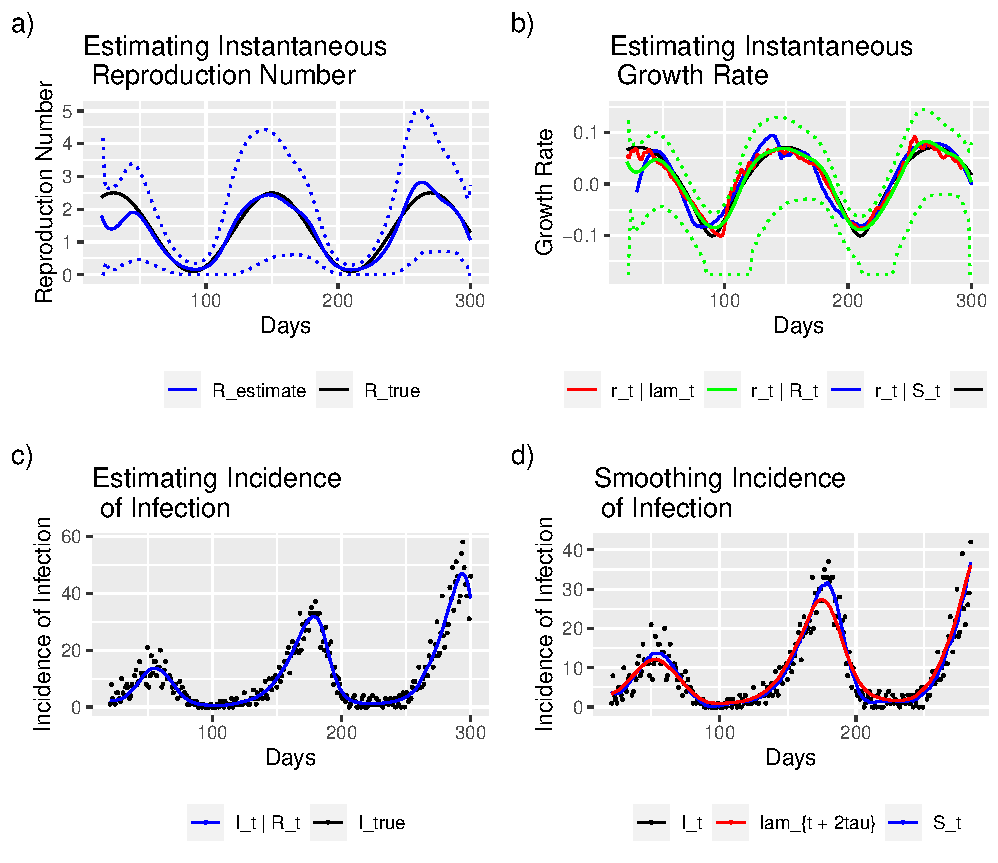
\includegraphics[scale = 0.75]{epi_paper.pdf}
      \caption{We model $R_t$ as a sinusoidal moving epidemic. Plot a) shows $R_t$ modelled by \textit{rtestim} in blue with 95\% confidence bands. Plot b) shows $r_t$ estimated by 1. $\hat{R}_t$ and \cref{eq: rt-Rt} in green with 95\% confidence bands, 2. SG filter with time window 51 and cubic fit in blue, 3. $\Lambda_t$ as smoothing function in red. The latter 2 are right and left shifted respectively by $\frac{\tau}{2} = 4$ days. Plot c) shows incidence estimated from $\hat{R}_t$ through Poisson rate. Plot d) compares SG filter with $\Lambda_t$ right-shifted by 8 days.}
      \label{fig: paper}
    \end{figure}

    \paragraph{Example 2: Misspecified GTD} The first deviation from satisfactory conditions is to use a misspecified GTD, as done in PTD. 
    This is quite reasonable in reality as it is
    difficult to determine the GTD due to not observing true incidence and using cases as a proxy. 
    This is especially prominent early in an epidemic when there is a lack of data to estimate the GTD. 
    We would assume that the estimates for $R_t$ under these conditions would be poor because $\Lambda_t$ is dependent on the GTD. Since we are still
    using the true incidence, $\hat{R}_t$ should deviate from the true $R_t$. 
    In our case take $W^{misspec} \sim \text{Gamma}(2.7066, 2.7066 / 15.3 * 3)$, which has $\frac{1}{3}$ the expected value of the true GTD in \cref{fig: paper}. 
    
    In \cref{fig: misspec} we see that $\hat{R}_t$ is a very poor estimator,
    however $\hat{r}_t \ |\ \hat{R}_t$, i.e. $\hat{r}_t$ derived from misspecified GTD and the same (poor) $\hat{R}_t$ through \cref{eq: rt-Rt}, performs well. 
    Quantitatively, $D_{KL}(R, \hat{R}^{misspec}) \approx 425$ whereas $D_{KL}(R, \hat{R}) \approx 39$, an over tenfold difference, but $D_{MSE}(r, \hat{r}) \approx 0.11$ is close to $D_{MSE}(r, \hat{r}) = 0.07$. 

    \begin{figure}[h]
      \centering
      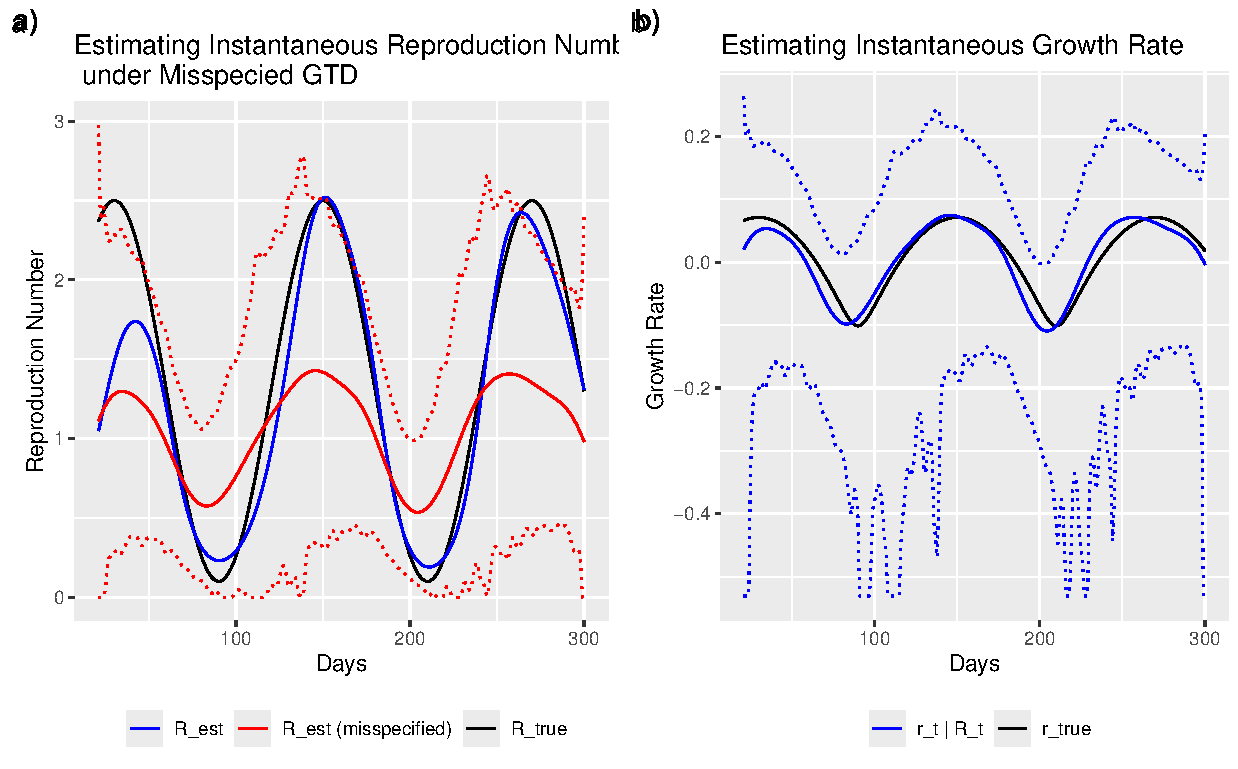
\includegraphics[scale = 0.6]{epi_misspec.pdf}
      \caption{We again model $R_t$ as an epidemic with sinusoidal movement. This time the GTD (gamma distribution) is misspecified. Plot a) shows $\hat{R}_t$ with well specified GTD in blue and misspecified GTD in red with 95\% confidence bands. Plot b) shows $\hat{r}_t$ estimated from misspecified $\hat{R}_t$ with 95\% confidence bands}
      \label{fig: misspec}
    \end{figure}

    \paragraph{Example 3: Piecewise Constant Epidemic} A practical situation of great importance to epedimiologists and policymakers is how $R_t$ changes with the implementation of various policies. 
    Consider a practical scenario where we have a baseline $R_t = 2$ for $t = 1,\dots,100$ in an epidemic, then a lockdown is instituted since infection rates are high and the rate goes down to 
    $R_t = 0.7$ for $t = 101,\dots,200$. After another 100 days infections are decreasing and so restrictions are lifted and the rate rises again to $R_t = 1.3$ 
    for $t = 201,\dots,300$. In reality, there will be some lag when policies are implemented, but we assume these changes have immediate effect and so 
    $R_t$ is a piecewise constant function. 
    
    \cref{fig: pc} shows the estimated $\hat{R}_t$ using \textit{rtestim}, using both piecewise cubic and piecewise constant functions 
    in the estimation. As expected, the piecewise constant models $R_t$ better, especially at jump points, due to the true $R_t$ being piecewise constant as well. We know this due to it being simulated data, however in practice, it can be difficult to determine what degree polynomial to fit. Quantitatively, $D_{KL}(R_0^{pc}, \hat{R}_0^{pc}) \approx 11$ whereas $D_{KL}(R_3^{pc}, \hat{R}_3^{pc}) \approx 36$.
    We also note that growth rate (all methods of estimation) models piecewise constant well but is naturally prone to jumpiness due to variation in incidence.

    \begin{figure}[h]
      \centering
      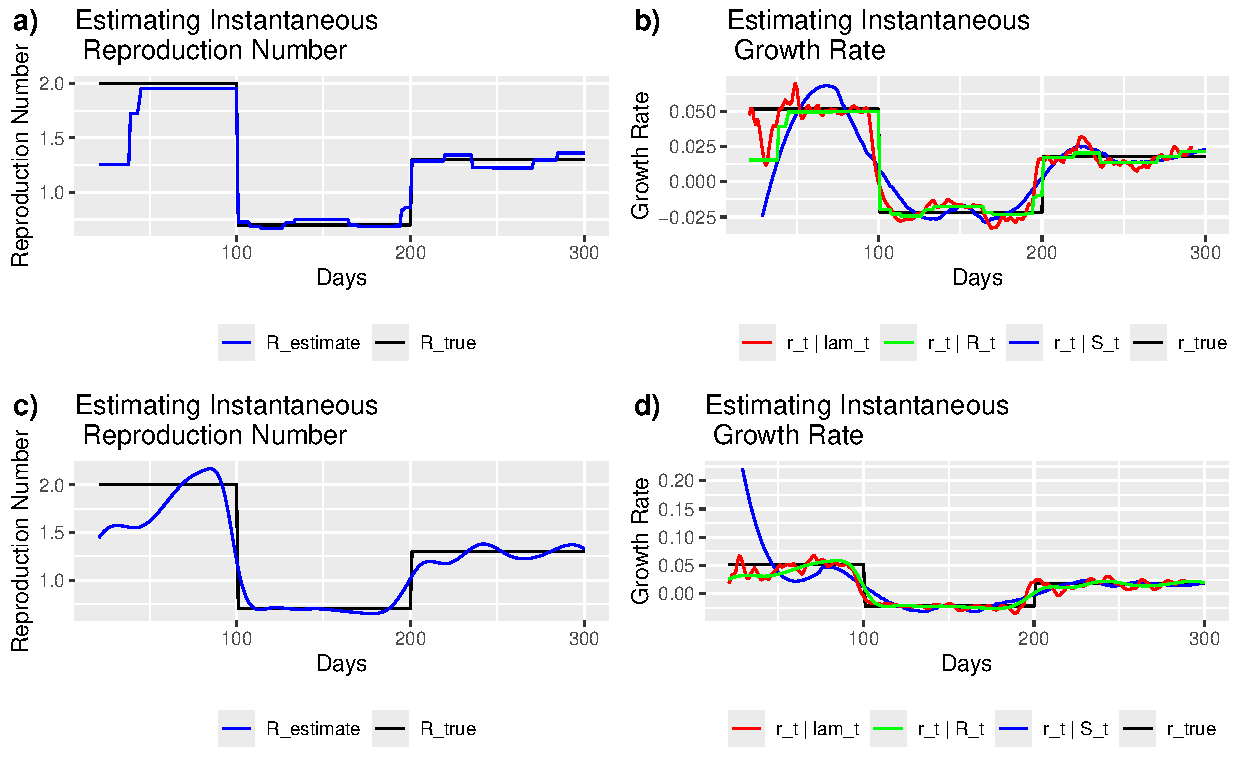
\includegraphics[scale = 0.75]{epi_pc.pdf}
      \caption{We model $R_t$ as a piecewise constant epidemic. Plots a) and c) shows $\hat{R}_t$ estimated with piecewise constant and piecewise cubic functions respectively in blue. Plots b) and d) show growth rate estimated in 3 ways.}
      \label{fig: pc}
    \end{figure}
    
    \paragraph{Example 4: Composite Epidemic} Consider next a slight modification of the previous scenario. Now in the first 100 days, $R_t$ is fluctating (modeled with sine wave) but upwards trending, followed
    by the implementation of a lockdown, which drops $R_t$ to a constant rate for the next 100 days. Then as restrictions gradually phase out (rather than all at once), 
    $R_t$ starts growing at a slow exponential rate. We model this with equation \cref{ex: lockdown}
    \begin{equation} \label{ex: lockdown}
      R_t = \left( \frac{t}{200} + \sin{\frac{\pi t}{20}} + 1.5 \right)\mathbf{1}_{1 \leq t \leq 100} + 0.8 \mathbf{1}_{100 < t \leq 200}
      + 0.08 e^{0.005 (t - 200)} \mathbf{1}_{200 < t \leq 300}
    \end{equation}

    Figure \cref{fig: comp} shows $\hat{R}_t$ and $\hat{r}_t$ estimates using piecewise cubic and linear estimators. They have respective KL divergences of $D_{KL}(R_1^{comp}, \hat{R}_1^{comp}) \approx 16$ and $D_{KL}(R_3^{comp}, \hat{R}_3^{comp}) \approx 25$. Though these are low values, neither can completely capture the epidemic movement because
    we simulated a true $R_t$ that is composed of an upward trending sine wave, constant, and slow growing exponential. The first part is better
    captured by the cubic spline since it has curvature, but the latter two components are better estimated by piecewise linear splines. In the same
    way, estimating $\hat{r}_t$ with SG filters does not model this example well. $\hat{r}_t$ estimates will always be jumpy because incidence is variable, 
    and there is no smoothing on the parameters (see \cref{eq: rt}), an issue that is exacerbated when the underlying growth rate is constant. This shows an opportunity to further develop methodologies that account for different epidemic movement patterns for long-run diseases.
    \begin{figure}[h]
      \centering
      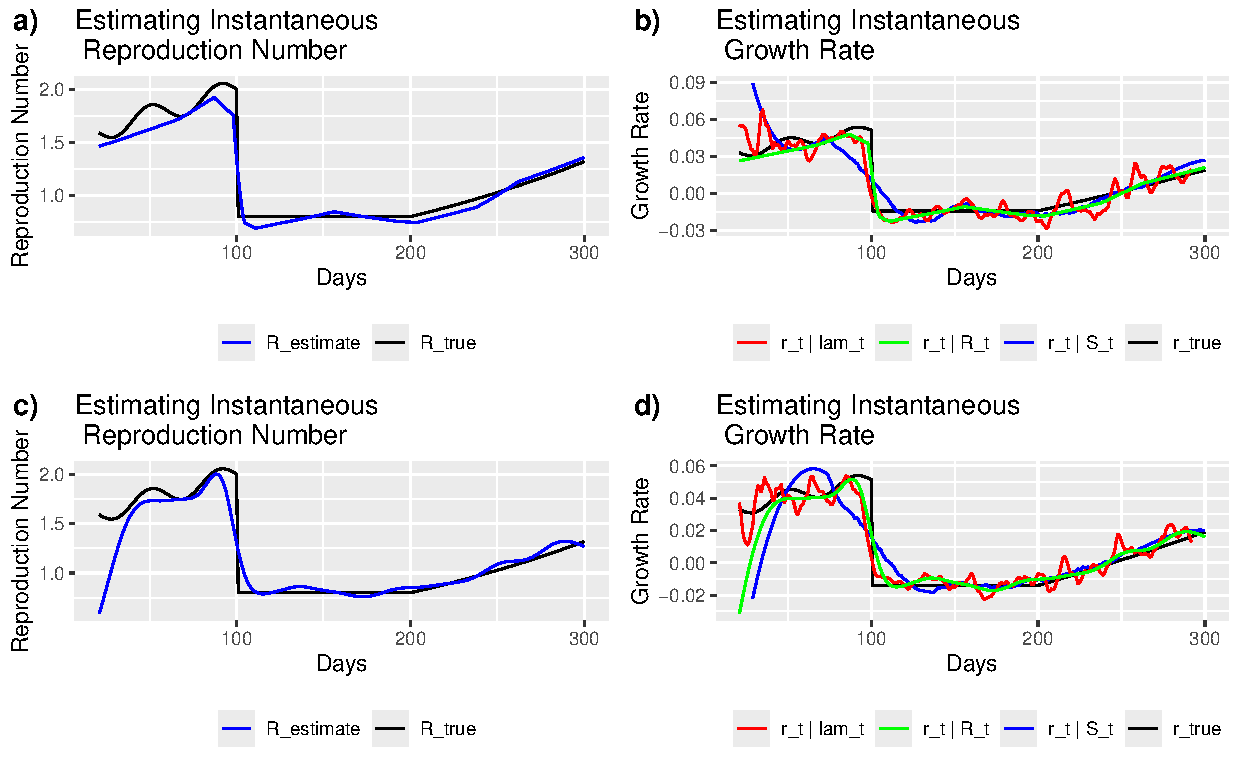
\includegraphics[scale = 0.75]{epi_comp.pdf}
      \caption{We model $R_t$ as a composite epidemic of upward trending sine wave, constant, and slow exponential growth. Plots a) and c) shows $\hat{R}_t$ estimated with piecewise linear and piecewise cubic functions respectively in blue. Plots b) and d) show growth rate estimated in 3 ways.}
      \label{fig: comp}
    \end{figure}
        
  \newpage

  \section{Appendices}

    \subsection{A1: Bayes Estimate for $\hat{R}_t$} \label{app: bayes}
      We wish to estimate $\hat{R}_t$ as in PTD. This derivation comes from the work in \citep{Cori2013}. 

      We assume that for each $t = 1,\dots,T$, $R_t$ has $\text{Gamma}(\alpha, \beta)$ prior, and conditional on previous incidence and $R_t$, $I_t$ is Poisson distributed with rate $\Lambda_t R_t$.
      This gives the probabiliities
      \[ \pi(R_t) = \frac{\beta^\alpha}{\Gamma(\alpha)} R_t^{\alpha - 1}e^{-\beta R_t} \quad 
      f(I_t \ |\ I_1,\dots,I_{t - 1}, R_t, W) = \frac{(\Lambda_t R_t)^{I_t} e^{-\Lambda_t R_t}}{I_t!} \]
      We then get the posterior probability
      \[
        \pi(R_t \ |\ I_1,\dots,I_t, W) &\propto \pi(R_t)f(I_t \ |\ I_1,\dots,I_{t - 1}, R_t, W) \\
        &\propto R_t^{\alpha - 1}e^{-\beta R_t} (\Lambda_t R_t)^{I_t} e^{-\Lambda_t R_t} \\
        &= \Lambda_t^{I_t}R_t^{\alpha + I_t - 1} e^{-(\beta + \Lambda_t)R_t}
      \]
      Thus we get that the posterior distribution of $R_t$ is also Gamma distributed with parameters
      \[ R_t \sim \text{Gamma}(\alpha + I_t, \beta + \Lambda_t) \]
      In particular, we estimate $\hat{R}_t$ as the posterior mean
      \[ \hat{R}_t = \frac{\alpha + I_t}{\beta + \Lambda_t} \]

    \subsection{A2: Connecting $\hat{R}_t$ and $\hat{r}_t$} \label{app: rtRt} 
      We wish to derive \cref{eq: rt-Rt}. This derivation comes from work in \citep{WallingaLipsitch2006} originally meant to model birth rates. 

      We assume that the number of infections at each time $t$ is simply the the infection at time $t - i$ times the rate of infection with lag $t - i$.
      \[ I_t = \sum_{j = 1}^\infty I_{t - j}n_j \]
      This is simply total infectiousness over infinite time. Moreover, we assume a crude form of exponential growth for $t = 1,2,\dots$.
      \[ I_t = I_{t - j}e^{jr_t} \]
      Lastly, we let $R_t$ be the total infectiousness of an individual over their lifetime, which is the sum of rates.
      \[ R_t = \sum_{j = 1}^\infty n_j \]
      Though this is an infinite sum, we can safely assume that $n_j \to 0$ since an individual will not remain infectious forever. It follows that $R_t$ is
      also the normalizing constant to turn rate $\{n_j\}_{j = 1}^\infty$ into a probability mass $\{w_j\}_{j = 1}^\infty$. That is $w_j = \frac{n_j}{R_t}$.
      Putting these equations together we get that.
      \[ I_t = \sum_{j = 1}^\infty I_{t - j}n_j &\implies I_t = \sum_{j = 1}^\infty I_t e^{-jr_t} R_t w_j \\
      &\implies \frac{1}{R_t} e^{-jr_t} w_j = \mathbb{M}_w(-r_t) \\
      &\implies 1 = R_t \mathbb{M}_w(-r_t) \]
      This is exactly \cref{eq: rt-Rt}. Note, that in the derivation, we do not actually depend on the time $t$, and so this holds for all $t = 1,\dots,T$.
      

    \subsection{A3: Smooth estimation of $\hat{r}_t$} 
      \begin{figure}[h]
        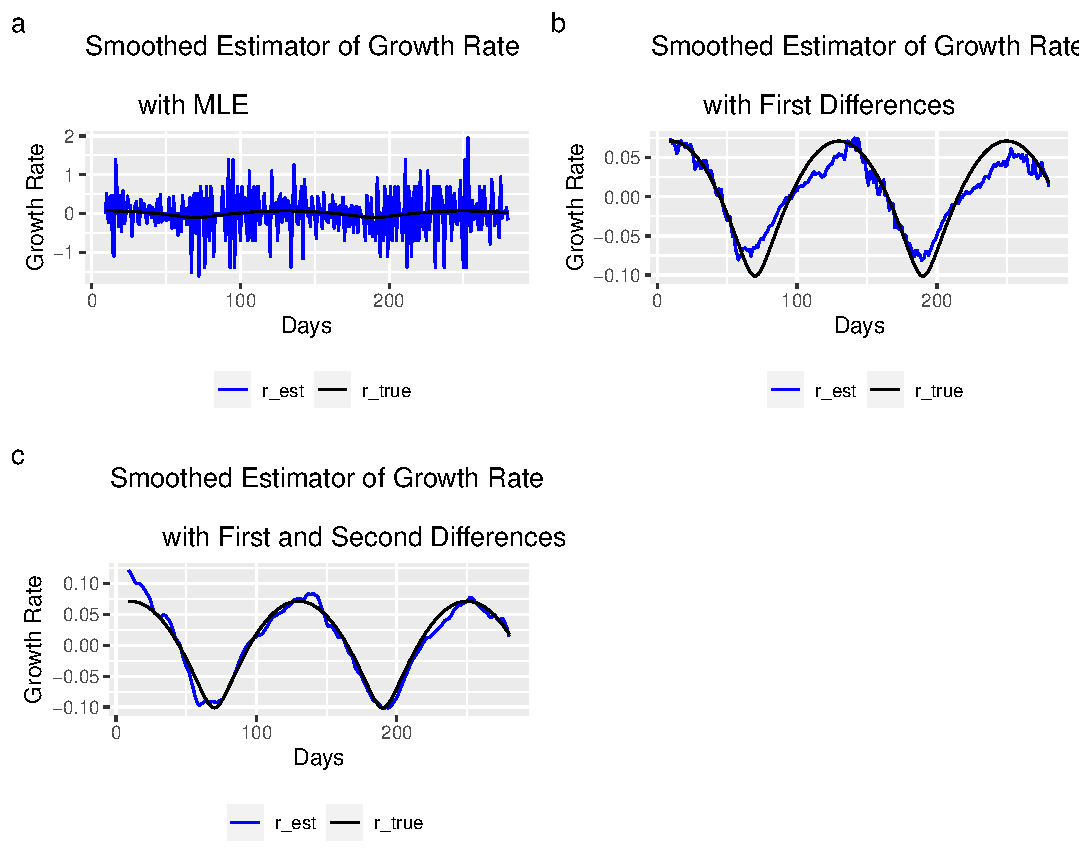
\includegraphics[scale = 0.75]{estimate_growthrate.pdf}
        \caption{We estimate $\hat{r}_t$ using maximum likelihood and penalized likelihood (in blue). plot a) shows estimation with MLE, plot b) adds a first differences penalty to likelihood in the estimation, and plot c) further adds second differences as a second penalization term in the estimation.}
        \label{fig: smoothrt}
      \end{figure}

    \subsection{A4: Convexity of Objective in smooth $\hat{r}_t$} \label{app: convex}
      We wish to show that the objective function is convex.
      \[\ell(r_1,\dots,r_t) = \sum_{t = 2}^T [I_{t - 1}e^{r_t} - I_t(\log{I_{t - 1}} + r_t)]
         + \sum_{t = 3}^T [\lambda_1 e^{(r_t - r_{t - 1})^2} + \lambda_2 e^{(r_t - 2r_{t - 1} + r_{t -2})^2}] \]
      Since the sum of convex functions is also convex, it suffices to show that each of its components is convex. To that end, consider an 
      arbitrary index $t$. $I_{t - 1}e^{r_t} - I_t(\log{I_{t - 1}} + r_t)$ is the sum of an exponential, constant, and linear function in $r_t$,
      all of which we know to be convex from univariate analysis. To see $e^{(r_t - r_{t - 1})^2}$ is convex, note that it has hessian of the form
      \[ H_1 = \begin{pmatrix} A & -A \\ -A & A \end{pmatrix}, \quad A = 4e^{(r_t - r_{t - 1})^2}(r_t - r_{t - 1})^2 + 2e^{(r_t - r_{t - 1})^2} \]
      $det(H_1) = 2A^2 \geq 0$ and so $H_1$ is positive semidefinite, which implies $e^{(r_t - r_{t - 1})^2}$ is convex.

      Similary for $e^{(r_t - 2r_{t - 1} + r_{t -2})^2}$, we have 
      \[ H_2 = \begin{pmatrix} A & -2A & A \\ -2A & 4A & -2A \\ A & -2A & A \end{pmatrix}, 
      \quad A = 4e^{(r_t - 2r_{t - 1} + r_{t -2})^2}(r_t - 2r_{t - 1} + r_{t -2})^2 + 2e^{(r_t - 2r_{t - 1} + r_{t -2})^2} \]
      $det(H_2) = 0$ and the eigenvalue of $H_2$ are 0 and 6, and so $H_2$ is positive semidefinite, which implies $e^{(r_t - 2r_{t - 1} + r_{t -2})^2}$ is convex. 
      We can conclude that the objective function is convex, as desired.


      \newpage 

\bibliographystyle{rss}
\bibliography{qp.bib}

\end{document}
